\documentclass{ximera}

\graphicspath{  %% When looking for images,
{./}            %% look here first,
{./pictures/}   %% then look for a pictures folder,
{../pictures/}  %% which may be a directory up.
}

\title{Setup a GitHub repository}

\author{Bart Snapp}

\begin{document}
\begin{abstract}
  How to set up your Ximera files in GitHub.
\end{abstract}
\maketitle

\textbf{All Ximera files must be hosted in a Git repository.} You have two
choices when creating new content:
\begin{itemize}
  \item If you are starting fresh, fork the \texttt{ximeraFirstSteps}
        repository.
  \item If you are starting with an existing a Git repository, move files
        from \texttt{ximeraFirstSteps} to this repository.
\end{itemize}

\section{Starting fresh and forking \texttt{ximeraFirstSteps}}

Forking a repository is well-documented on
\link[GitHub]{https://docs.github.com/en/pull-requests/collaborating-with-pull-requests/working-with-forks/fork-a-repo}.
Basically, you login to GitHub, return to this page, and at the top right there
will be an option to `Fork' this repository. Fork the repo. Accept all
defaults, though you might want to change the name of the repository at this
point. When done, it will take you to
your copy of this repository on GitHub. It will be located someplace like:
\begin{center}
  \texttt{https://github.com/YOUR-GIT-USER-NAME/your-new-repo-name}
\end{center}
Once the repository is forked, clone the forked repository (the one in your
user-space) onto your computer. \textbf{If you are using Windows, be sure to
  clone through WSL.}
After the repository is on your computer, delete all files \textbf{except:}
\begin{itemize}
  \item \texttt{.gitignore}
  \item \texttt{DOTximeraserve}
  \item \texttt{.vscode}
  \item \texttt{scripts}
  \item \texttt{.git}
  \item \texttt{README.md}
  \item \texttt{NOT-THE-LICENSE.md}
\end{itemize}
You must keep the files above.	Commit your changes to GitHub and view your
repository online via a web browser to ensure that the files were deleted.

\section{Starting from an existing GitHub repository}

Starting from an existing GitHub repository, you will need to \textbf{copy}
\begin{itemize}
  \item \texttt{gitignore}
  \item \texttt{.vscode}
  \item \texttt{scripts}
  \item \texttt{README.md}
  \item \texttt{NOT-THE-LICENSE.md}
\end{itemize}
into your repository. If you already have a \verb|.gitignore| file, we suggest
you replace yours with ours. Commit your changes to GitHub and view your
repository online via a web browser to ensure that the files were added.

\section{Setting up a Ximera \texttt{xourse}}

Ximera documents can be ``taped'' together using the \texttt{xourse} document
class.
A \verb|xourse| file is basically a list of other \verb|ximera| files and even
other \verb|xourse| files.
The \verb|xourse| file for \textit{First Steps in Ximera} can be found here:
\begin{center}

  \url{https://github.com/ximeraProject/ximeraFirstSteps/aFirstStepInXimera.tex}
\end{center}

This gets complicated because we insist that Ximera documents must compiled not
only when in a \verb|xourse| file, but also individually.
\begin{center}
  \resizebox{!}{5cm}{
  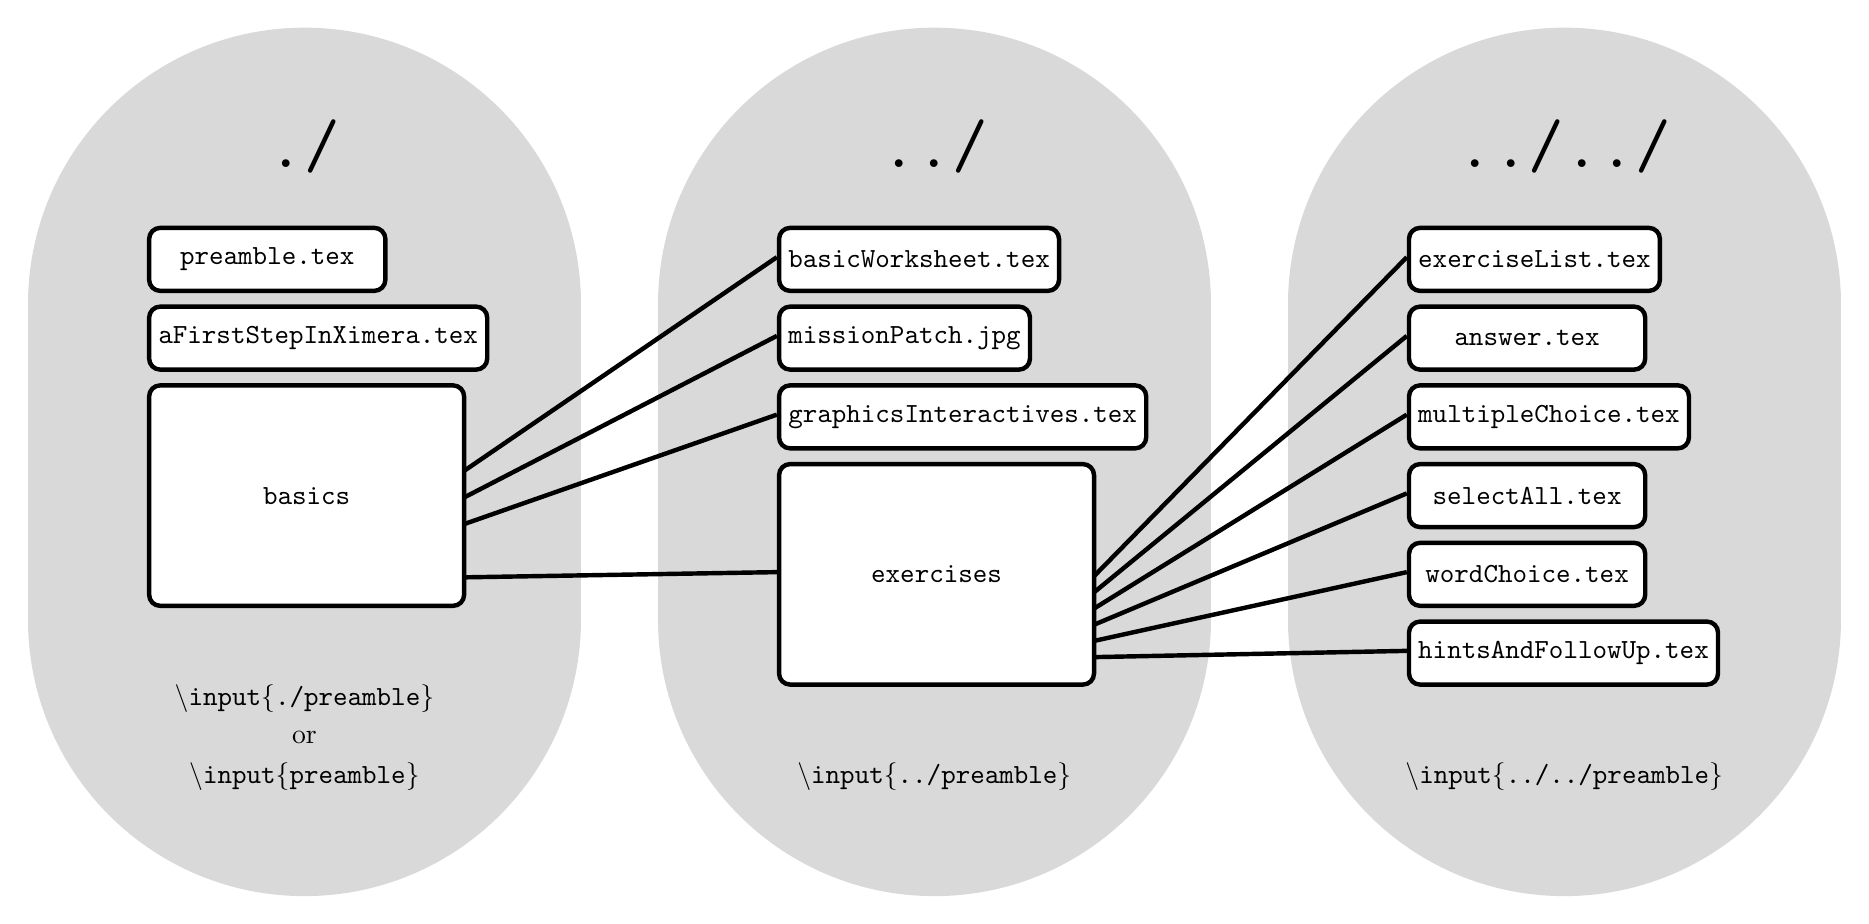
\begin{tikzpicture}
    % Define styles for nodes
    \tikzstyle{document} = [anchor=north west,draw, rounded corners, rectangle,
    minimum width=3cm,fill=white, minimum height=.8cm, ultra
    thick,font=\ttfamily]
    \tikzstyle{folder} = [anchor=north west,draw, rectangle, rounded corners,
    minimum width=4cm,fill=white, minimum height=2.8cm, ultra
    thick,font=\ttfamily]

    % Thick grey lines
    \draw[line width=200pt,white!85!black,line cap=round] (2,2) -- (2,-2);
    \draw[line width=200pt,white!85!black,line cap=round] (10,2) -- (10,-2);
    \draw[line width=200pt,white!85!black,line cap=round] (18,2) -- (18,-2);

    % Connections
    \draw[ultra thick] (2,-1.5) -- (8,2.6);
    \draw[ultra thick] (2,-1.5) -- (8,1.6);
    \draw[ultra thick] (2,-1.5) -- (8,.6);
    \draw[ultra thick] (2,-1.5) -- (8,-1.4);

    \draw[ultra thick] (11,-2.5) -- (16,2.6);
    \draw[ultra thick] (11,-2.5) -- (16,1.6);
    \draw[ultra thick] (11,-2.5) -- (16,.6);
    \draw[ultra thick] (11,-2.5) -- (16,-.4);
    \draw[ultra thick] (11,-2.5) -- (16,-1.4);
    \draw[ultra thick] (11,-2.5) -- (16,-2.4);

    % Symbols at top
    \node at (2,4) {\Huge \tt ./};
    \node at (10,4) {\Huge \tt ../};
    \node at (18,4) {\Huge \tt ../../};

    % Define the folders at top level
    \node[document] at (0,3) {preamble.tex};
    \node[document] at (0,2) {aFirstStepInXimera.tex};
    \node[folder] at (0,1) {basics};

    % Define the documents in the basics folder
    \node[document] at (8,3) {basicWorksheet.tex};
    \node[document] at (8,2) {missionPatch.jpg};
    \node[document] at (8,1) {graphicsInteractives.tex};
    \node[folder] at (8,0) {exercises};

    % Define the documents in the exercises folder
    \node[document] at (16,3) {exerciseList.tex};
    \node[document] at (16,2) {answer.tex};
    \node[document] at (16,1) {multipleChoice.tex};
    \node[document] at (16,0) {selectAll.tex};
    \node[document] at (16,-1) {wordChoice.tex};
    \node[document] at (16,-2) {hintsAndFollowUp.tex};

    % paths at bottom
    \node at (2,-3) {\tt\textbackslash input\{./preamble\}};
    \node at (2,-3.5) {or};
    \node at (2,-4) {\tt\textbackslash input\{preamble\}};
    \node at (10,-4) {\tt\textbackslash input\{../preamble\}};
    \node at (18,-4) {\tt\textbackslash input\{../../preamble\}};
\end{tikzpicture}}
\end{center}

In general the file with the \verb!xourse! document class specifies
course information such as the name of the course, a description of
the course, and the names of all \LaTeX\ activity files comprising
the
course, in the order they should be presented to students.  In
addition to a name and a description, \verb!anExampleCourse.tex!
above specifies that there is one activity file
\verb!theFirstActivity.tex!, written with or without the extension
\verb!.tex!, and located in a directory called
\verb!theFirstActivity!.  We will create this file and directory in
the following

Generally courses should contain more than one activity. We recommend placing
each activity in a directory of the same name.	  This facilitates sharing
activities among collaborators and makes reusing existing activities easier.
%Later in this course, we will see examples of %how to borrow existing activities from other courses %rather than starting from scratch. We also recommend that the directory and the \LaTeX\ file have exactly the same name as the title of the activity, with all spaces removed and all words other than the first word capitalio for example, if the title of the activity were \verb!Plants native to Ohio!
the \LaTeX\ file \verb!plantsNativeToOhio.tex!
would be located in a directory called
\verb!plantsNativeToOhio!.

An activity should be composed as a regular \LaTeX\ file in the document class
\verb!ximera!. It should contain the title of the activity and an abstract.
These will both appear on the course website in the navigation area, so the
abstract should be short. At this stage your activity contains a title and an
abstract, but is otherwise blank.

Type \verb!xake bake! to compile the tex documents, then
\verb!xake frost! to create a publication commit on top of your source
commit.
Finally type \verb!xake serve! to share your content with the world.
For
instance, my content will appear at
https://ximera.osu.edu/turnloon/anExampleCourse

This is a good point to add some further content in the
form of a simple exercise.  Update the file
\verb!theFirstActivity.tex!  you created above so that it looks like
the following.

\subsection{Creating further activities}
From here you can create further \link[Ximera]{http://ximera.osu.edu}
activities as in step~\autoref{FirstExercise}.	You should issue a
\verb!git add! command after creating a new file or directory and a
\verb!git commit!  command followed by a \verb!git push! command
periodically to transmit your most recent changes to
\link[github.com]{http://github.com}.  You should also add the name of
your activity file to the \verb!xourse! file in the position relative
to other activities where you want the activity to appear.  Observe
however that once the filename appears in the \verb!xourse!  file the
corresponding activity will appear to students. It might therefore be
preferable to create a separate branch on GitHub until the activity is
ready for students.  During the editing phase you still view the
activity by processing it with \LaTeX\ and inspecting the resulting
PDF file, which might be helpful in any case for finding and
correcting mistakes.

\subsection{Other ways to set up a Ximera repository}\label{ForkClone}
There are other ways to create a \link[Ximera]{http://ximera.osu.edu}
course.  One possibility is to begin by creating the repository on
\link[github.com]{http://github.com}.  Then instead of executing the commands
to
initialize the local copy of the repository, you could {\em clone} the
copy on \link[github.com]{http://github.com} using a \verb!git clone!
command.  Alternately you could {\em fork} an existing repository,
either your own or someone else's.  See the \link[git
  manual]{http://git-scm.com} for more information about the
\verb!clone! and \verb!fork! commands.	Both possibilities above
obviate step \autoref{Mkdir} since cloning or forking a
\link[git]{http://git-scm.com} repository creates a local directory
and initializes it as a \link[git]{http://git-scm.com} repository.

\end{document}